\documentclass[12pt]{article}					% Začátek dokumentu
\usepackage{../../MFFStyle}							% Import stylu

\begin{document}
\begin{priklad}
	A dice is rolled repeatedly. Which of the following are Markov chains? For those that are, supply the transition graph.

	\begin{itemize}
		\item $M_t$ is the largest number shown on the dice up to the $t$-th roll.
		\item $N_t$ is the number of sixes in first $t$ rolls.
		\item $A_t$ is the time since (“after”) the most recent six. (So $A_t = 0$ when the $t$-th roll was a six, $A_t = 1$ when $(t−1)$-st was a six, but not the $t$-th, etc.
		\item $B_t$ is the time before the next six.
(So $B_t = 0$ when the $t$-th roll was a six, $B_t = 1$ when $(t+1)$-st was a six, but not the $t$-th, etc.
	\end{itemize}

	\begin{reseni}
		All of them are Markov chains. Graphs are made with \url{https://mxwell.github.io/draw-graph/}.
	\end{reseni}

	\begin{reseni}[The transition graph for the first one]
		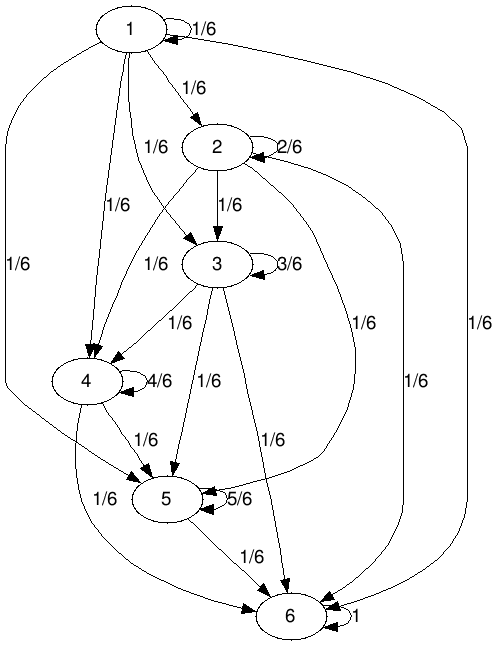
\includegraphics[width=0.5\textwidth]{chart.png}
	\end{reseni}
		
	\begin{reseni}[The transition graph for the second one]
		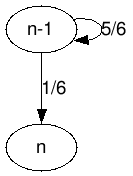
\includegraphics[width=0.1\textwidth]{chart2.png}
		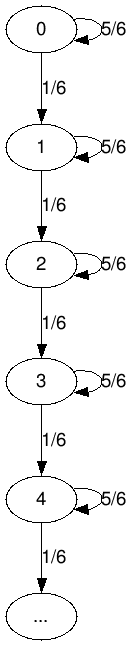
\includegraphics[width=0.1\textwidth]{chart2B.png}
	\end{reseni}

	\begin{reseni}[The transition graph for the third one:]
		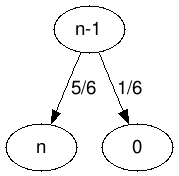
\includegraphics[width=0.2\textwidth]{chart3.png}
		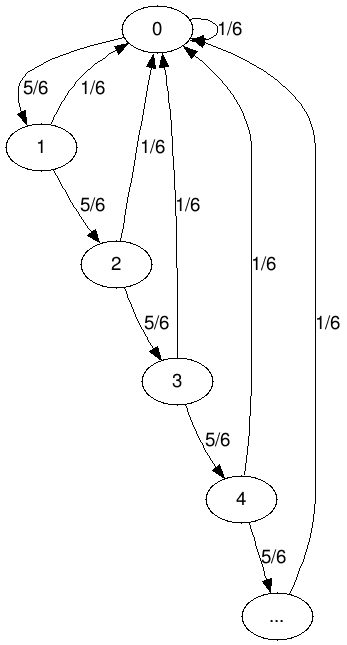
\includegraphics[width=0.3\textwidth]{chart3B.png}
	\end{reseni}

	\begin{reseni}[The transition graph for the fourth one:]
		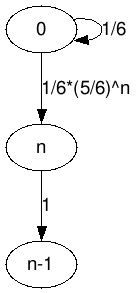
\includegraphics[width=0.1\textwidth]{chart4.png}
		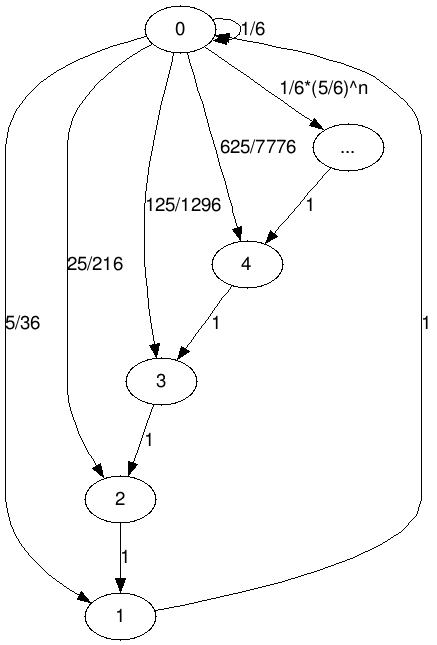
\includegraphics[width=0.4\textwidth]{chart4B.png}
	\end{reseni}
\end{priklad}



\end{document}
